% !TEX root = quickstep.tex
\chapter{Design and Implementation of Quickstep System}

\section{Introduction}
Query processing systems today face a host of challenges that were not as prominent just a few years ago. A key change has been dramatic changes in the hardware landscape that is driven by the need to consider energy as a first-class (hardware) design parameter. Across the entire processor-IO hierarchy, the hardware paradigm today looks very different than it did just a few years ago. Consequently, we are now experiencing a growing \textit{deficit} between the pace of hardware performance improvements and the pace that is demanded of data processing kernels to keep up with the growth in data volumes.

%\begin{figure}
%\centering
%   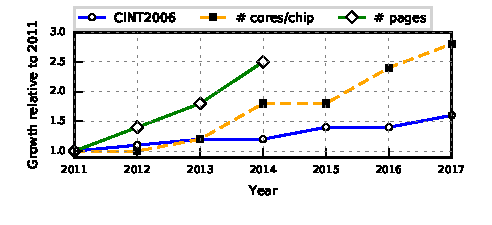
\includegraphics[width=\columnwidth]{system/figures/deficit.pdf}
%   \vspace*{-2em}
%   \caption{\textbf{Processor performance improvement as measured by the highest reported CINT2006 benchmark result for Intel Xeon chips from~\cite{cpu2006} compared to the number of pages indexed by Google (using estimates made by~\cite{google-pages-db}). The figure does not show the increase in the number of queries (which is about 2.5X for Google search queries from 2011--14), and the increase in the complexity of queries as applications request richer analytics. These aspects make the deficit problem worse. The figure also shows the maximum number of cores per chip used in reported CINT2006 results over time. Interestingly (and not shown in the figure), both the minimum and the average amount of memory per chip in the reported CINT2006 results has grown by $\approx$4X from 2011 to 2017.}}
%   % For example, the number of Google search queries has gone up by a factor of 6X in the time period shown in the graph above.}
%   \label{fig-deficit}
%\end{figure}

Figure~\ref{fig-deficit} illustrates this deficit issue by comparing improvements in processor performance (blue line) with the growth rate of data (green line), using the number of pages indexed by Google as an illustrative example. This data growth rate is conservative for many organizations, which tend to see a far higher rate of increase in the data volume; for example, Facebook's warehouse grew by 3X in 2014~\cite{fb-growth-14}. This figure also shows (using a dotted orange line with squares) the growth in the number of cores per processor over time. As one can observe, the number of cores per processor is rising rapidly. % as multi-core parallelism is critical for processor vendors.
%to realizing overall higher processor performance.
%(While we do not consider this further in this paper, the number of cores per processing unit is even higher for non-traditional processors/co-processors.)
% Thus, the demands on query processing can't simply be met by only throwing more chips/processors at the problem.
%Thus, there is a critical need for systems that can exploit the full potential of the hardware parallelism that is available in each box.
In addition, %as noted in the caption of the figure,
since 2011 the main memory sizes are also growing rapidly, and there is an increasing shift to larger main memory configurations. Thus, there is a critical need for in-memory data processing methods that \textit{scale-up} to exploit the full (parallel) processing power that is  locked in commodity multi-core servers today. \Quickstep\ targets this need, and in this paper we describe the initial version of Quickstep that targets single-node %settings, and for the important case of
in-memory read-mostly analytic workloads.


%The deficit/difference between the data and query growth rates compared to the raw hardware performance is unsustainable in the long run. One way to ``pay off'' this deficit is to have hardware and software co-evolve to exploit the full potential of the hardware. Thus, a key thrust behind this current, initial, phase of the \Quickstep\ project, is to develop data processing kernels (e.g. implementation of selection, join, and aggregation operator algorithms) that can run efficiently on contemporary hardware, and to find ways to compose them efficiently to answer more complex queries. This line of thinking can be considered as \textit{scaling-up} to exploit the (parallel) processing power that is  locked in commodity servers today.


%The second big challenge for data analytics platform today is to rethink the performance metric that is used to evaluate queries. Traditional metrics such as query throughput and query latency are still important, but not as important as p9X values (e.g. thep95 query latency values). Even robust commercial systems today do fairly poorly on this metric, as illustrated in Figure 2. So, why are p9X metrics more valuable than using average as a metric? The reason is that data processing systems are generally run on cluster, in which tail latencies~\ref{tail-at-scale} are common, and severely impact the responsive of the applications/services that are built on top of the data platform. Thus, for example, if dynamic content on a mobile app is created by executing queries against a database system, then it is far more important for the application developer to know that in 99\% of the queries the query latency will be below a certain values, say 100ms, than to know what the average query response time is. Similarly, to serve up real-time analytics, one cares more about predicable query response time~\ref{constant-query-time} play a crucial role in actual deployments that tend to use data platforms to serve up responses to end users

%We also note that there are a few additional technological trends. One important trend is a shift in many data analytics environments to read-mostly settings. (For this paper, data analytics is broadly defined to encompass query processing in data warehousing environments.) In such settings, data is loaded into a ``warehouse'' and is not updated in-place. Rather, new data is appended to an existing database. This shift can be seen by the huge interest in moving analytical SQL workloads to Hadoop-based systems like  Drill~\cite{drill}, HAWQ~\cite{hawq}, Hive on Tez~\cite{Tez}, Impala~\cite{impala},  and Spark~\cite{Spark}. Since many of these systems are built on top of the Hadoop Distributed File System (HDFS), and since HDFS is append-only, these systems naturally have to live with this read-mostly constraint. But, it turns out that other warehouse scenarios are also amenable to this paradigm of read-mostly setting.
%(The community-driven open-source model and lower initial cost to set up a warehouse are other factors that have propelled the interest in SQL-on-Hadoop systems.)

%Another trend is the continuing need for high  performance on in-memory analytic workloads. The focus on performance is driven by a number of factors, including closer integration of data analytics with decision-making in enterprises, which naturally leads to a demand for interactive analytics. Performance is also critical as the move to cloud settings (both public and private clouds) has made ``accountability'' a bigger emphasis for users of the analytics systems. For example, when running analytics in a public cloud, higher performance translates to lower monetary cost for running the data analytics service. Even when running in private clouds, there is an increasing trend to monitor the usage of the cloud resources for groups within the enterprise, and to ``bill'' each group to create increased awareness about the costs that each group is incurring.

%In addition, large main memory configurations are now common and affordable. Commodity servers with tens to hundreds of gigabytes of DRAM are increasingly economical. Memory densities are predicted to continue to grow over the upcoming decade, and fully or mostly in-memory processing is increasingly common for many analytical applications. This technological trend has led to the resurgence of main memory databases and has pushed in-memory computing to the forefront of data analytics products that are offered today.

%A natural question is whether the changing patterns listed above require rethinking how to build modern analytical query processing systems. In this paper we describe a system, called Quickstep, that explores these issues for the important case of in-memory settings and read-mostly analytic workloads.
%We have built a single-node version of the system, which we describe in this paper. This initial version targets in-memory settings and read-mostly analytic workload (similar to systems such as Spark~\cite{Spark}).
%A key contribution of our paper is to present the end-to-end design of Quickstep.

%Another critical contribution, which is subtle but we believe is important, is making the entire system available as open-source. We note that our community has attempted to take reproducability seriously~\cite{BonnetMBCGGHIIJKKMOPRTYFS11, ManegoldMAFGHHKKLLORSSWS09, ManolescuAADMPSSZS08}, which is naturally easier to achieve with open-source systems. However, open-sourcing a system goes beyond reproducability as it allows for \textit{transparency} that permits a deeper understanding of the end-to-end system effects. This aspect is especially critical when working on research problems where the impact of specific techniques is important only when cast within the context of the overall system behavior.

%Next, we describe key aspects of the Quickstep system.
To pay off the deficit, Quickstep
%have taken the approach of thinking bottom-up from the hardware to the software. A crucial design is to
uses mechanisms that allow for \textit{high intra-operator parallelism}. Such mechanisms are critical to exploit the full potential of the high level of hardware compute parallelism that is present in modern servers (the dotted orange line in Figure~\ref{fig-deficit}).
%First, to deal with the new hardware reality, we have taken the approach of thinking bottom-up from the hardware to the software. This unique co-design approach naturally forces us to compare the raw performance of the hardware and the end performance delivered by data analytics software running on this hardware. We ask if there are technical mechanisms that can be developed to allow for the software to deliver bare-metal performance. A crucial aspect of \Quickstep\ is adopting the use of BitWeaving~\cite{bitweaving} as a way to store/index the data, so that scan queries, which are the workhorse operations in-memory analytical systems~\cite{SIMD-DBMS, RamanSQRDKNS08, JohnsonRSS08,WillhalmPBPZS09, WillhalmO0F13, QiaoRRHL08}, can run at bare-metal speeds.
%(\Quickstep\ also supports CSB+-tree~\cite{csbtree} indices.)
%Second,
Unlike most research database management systems (DBMSs), \Quickstep\ has a storage manager with a block layout, where each block behaves like a mini self-contained database~\cite{ChasseurP13}.
%Thus, any indices are packed in the block along with the actual tuple data.
%This design allows \Quickstep\ to easily transform data that is stored locally within a block to best suit the organization that maximizes query performance, and reduces the need for global coordination for physical schema changes. For example, data that is being loaded can be stored in a block that is in a row-store format, and that block can be morphed into a compressed row store with indices when it is full. % to speed up subsequent analytics queries.
This ``independent'' block-based storage design is leveraged by a highly parallelizable query execution paradigm in which independent \textit{work orders} are generated at the block level. Query execution then amounts to creating and scheduling work orders, which can be done in a generic way. Thus, the scheduler is a crucial system component, and the Quickstep scheduler cleanly separates scheduling policies from the underlying scheduling mechanisms. This separation allows the system to elastically scale the resources that are allocated to queries, and to adjust the resource allocations dynamically to meet various policy-related goals.


%This method of ``breaking down'' the query into work orders implies that at run time the data flow can be decoupled from the control flow. There is no upfront decision that is required to make decisions like the degree of intra-operator parallelism (even in a pipeline of query operators). Thus, the system has a high degree of freedom in executing tasks, which allows it to easily exploit the parallelism that is offered by contemporary multi-core, multi-socket machines.

%Second, \Quickstep\ uses a scheduler to make run-time decisions about query execution. Working with the block-based storage design allows the scheduler to make dynamic run-time decisions. This feature gives \Quickstep\ an high level of flexibility in allocating resources dynamically to deal with a variety of end goals, such as quickly shifting resources to  high-priority queries when they arrive. Such system behavior is very desirable in cloud environments when resources are shared and workload management requires the ability to deal with different query classes efficiently and effectively.

%Third, we use novel query processing techniques for high performance. The scan/select operations use BitWeaved indices (whenever possible) that are efficient for scans. \Quickstep\ also implements other relational operators, including hash-based joins and hash-based aggregation, and uses state-of-the-art parallel latch-free algorithms for these operators. In addition, a database in \Quickstep\ can be ``denormalized'' using WideTables~\cite{widetable}, which examines the schema to flatten the database into a set of denormalized tables that are materialized. With this approach, a large class of complex queries can be converted to (fast) scans on the WideTables; queries that can't be transformed are evaluated in the ``traditional'' way using the usual relational operations (including joins).

%Third, \Quickstep\ uses a \textit{template metaprogramming} technique to generate highly optimized code when accessing data residing in blocks. This method incurs only a one-time cost when building the \Quickstep\ binaries. This method of vectorization generates compact inner loops for expression and operator evaluation, which can be evaluated efficiently by modern processors (as the code generated is amenable to mechanisms like prefetching).

%Fourth, \Quickstep\ uses novel query processing techniques for high performance. In this paper we describe one such approach in detail that considers in-lining tuples inside hash tables to improve the performance of join operations.

Recognizing that random memory access patterns and materialization costs often dominate the execution time in main-memory DBMSs, Quickstep uses a number of query processing techniques that take the ``drop early, drop fast'' approach: eliminating redundant rows as early as possible, as fast as possible. For instance, Quickstep aggressively pushes down complex disjunctive predicates involving multiple tables using a %novel
predicate over-approximation scheme. Quickstep also uses cache-efficient filter data structures to pass information across primary key-foreign key equijoins,  eliminating semi-joins entirely in some cases. %, and optimally processing deep join trees. %We show that the combination of these techniques provides big improvements in performance.

%Quickstep also pushes on query processing techniques for complex pipelines of joins in main-memory environments. We present novel filter-based methods that dramatically improve the performance of a sequence of primary key-foreign key equijoins, which naturally appear quite frequently in analytic query processing environments.

% has not been well explored. There are many open questions about what traditional query optimization techniques apply in main-memory settings, and if new methods that are needed. We have explored some of these issues (and acknowledge that there is a lot more potential for future work). In this paper, we describe a set of \textit{join optimization techniques} to speed up typical queries containing sequences of join operations. %-- a pattern that is common in analytic query processing environments.

%Quickstep is designed to be easy to use in a variety of settings, including as a standalone server  and as an embedded database engine in virtualized containers. Quickstep employs a unified buffer manager to store both the database tables and any intermediate results (including hash tables that are built during query execution). In many database systems various memory knobs have to be ``set right'' for memory management. Quickstep does not require such tuning. Similarly, Quickstep automatically senses the parallelism in the hardware environment (number of cores) and uses this information to naturally set the degree of parallelism for query execution. Thus, Quickstep can be spun up in any standalone server/container, and the system auto-tunes to exploit the full parallelism potential in the underlying hardware.

%, it is really optimized for the case when the dataset fits in main memory. Thus, it aims to leverage the in-memory technological trend to produce a data analytics system that executes queries fast. %near the speed of the underlying hardware.

%Finally, we also present results from a comprehensive end-to-end evaluation that compares \Quickstep\ with a number of other existing systems (Spark, PostgreSQL, MonetDB and VectorWise). Our results show that \Quickstep\ is high performant, and in some cases is faster by an order-of-magnitude over existing systems.

\begin{figure}
	\centering
	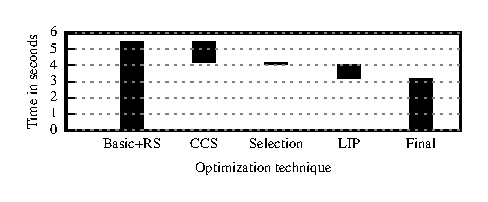
\includegraphics[width=0.5\textwidth]{system/figures/tpch-q10-waterfall.pdf}
	\caption{\textbf{A waterfall chart showing the impact of various techniques in Quickstep for query 10 from the TPC-H benchmark running on a 100 scale factor database. RS (Row Store), and CCS (Compressed Column Store) are both supported in Quickstep (see Section~\ref{block-structure}). Basic and Selection are template metaprogramming optimizations (described in Section~\ref{vectorization}), which relate to the efficiency of predicate and expression evaluation. LIP (Lookahead Information Passing, described in Section~\ref{sec:lip}) is a technique to improve join performance. Starting with a configuration (Basic + RS), each technique is introduced one at a time to show the individual impact of each technique on this query.}}
	\label{fig:tpch-q10-waterfall}
\end{figure}

Overall, the key contributions of this paper are as follows:\\
%\begin{itemize} [noitemsep,nolistsep]
\textbf{Cohesive collection of techniques:} We present the first end-to-end design for Quickstep. This system brings together in a single artifact a number of mechanisms for in-memory query processing such as support for multiple storage formats, a template metaprogramming approach to both manage the software complexity associated with supporting multiple storage formats and to evaluate expressions on data in each storage format efficiently, and novel query optimization techniques.
%The collection of these mechanisms result in overall high performance.
The impact of each mechanism depends on the workload, and our system brings these mechanisms together as a whole.
For example, the waterfall chart in Figure~\ref{fig:tpch-q10-waterfall} shows the contributions of various techniques on the performance of TPC-H Query 10.

\textbf{Novel query processing techniques:} We present Quickstep's use of techniques to aggressively push down complex disjunctive predicates involving multiple relations, as well as to eliminate certain types of equijoins using \textit{exact filters}.

%\item We generalize a recently proposed method (LIP) to speed up join processing.
\textbf{Manageability:} The design of the system focuses on ease-of-use, paying attention to a number of issues, including employing methods such as using a holistic approach to memory management, and elastically scaling query resource usage at runtime to gracefully deal with concurrent queries with varying query priorities.
%\item We also present a number of interesting query processing techniques including the use of embedded tuples in hash tables. In addition, we show how \Quickstep\ uses an interesting query optimization technique based on join filters to achieve high performance.

\textbf{Comparison with other systems:} We also conduct an end-to-end evaluation comparing \Quickstep\ with a number of other systems. These system are: Spark~\cite{Spark, SparkSQL}, PostgreSQL~\cite{postgres}, MonetDB~\cite{monetdb}, and VectorWise~\cite{vectorwise}. Our results show that in many cases, Quickstep is faster by an order-of-magnitude, or more.

% over some of these existing systems.

We also leverage the multiple different storage implementations in Quickstep to better understand the end-to-end impact of the popular row store and column store methods on the SSB and TPC-H queries. To the best of our knowkedge, an apples-to-apples comparison of these benchmark queries does not exist. We show that overall column stores are still preferred, though the speed up overall is only about 2X. Earlier comparisions, e.g.~\cite{AbadiMH08}, have been indirect comparisons of this aspect of storage management for the SSB benchmark across two different systems, and show far larger (6X) improvements. %We also find that overall for the SSB benchmark compression does not produce significant benefits.

\textbf{Open source:} Quickstep\ is available as open-source, which we hope helps the reproducability goal that is being pursued in our community~\cite{BonnetMBCGGHIIJKKMOPRTYFS11, ManegoldMAFGHHKKLLORSSWS09, ManolescuAADMPSSZS08}. It also allows other researchers to use this system as a platform when working on  problems where the impact of specific techniques can be best studied within the context of the overall system behavior.

%\end{itemize}
%We also make \Quickstep\ available as open-source. We note that our community has attempted to take reproducability seriously~\cite{BonnetMBCGGHIIJKKMOPRTYFS11, ManegoldMAFGHHKKLLORSSWS09, ManolescuAADMPSSZS08}, which is naturally easier to achieve with open-source systems. However, open-sourcing a system goes beyond reproducability as it allows for \textit{transparency} that permits a deeper understanding of the end-to-end system effects. This aspect is especially critical when working on research problems where the impact of specific techniques is important only when cast within the context of the overall system behavior.
% We consider this later part to be an important research contribution, not only because it allows easy reproduction of our results, but because it also has the potential to provide a baseline platform for research that aims to exploit the full potential of parallelism that is available inside modern servers.

%To keep the paper focused, we only consider in-memory settings.
%Given the overview nature of this paper and the space limitations, the evaluation component focuses on the broader end-to-end evaluation. There are interesting experiments that could be carried out for individual components and some of our past papers have explored some of these choices individually (e.g.~\cite{bitweaving, LiCP15, ChasseurP13, widetable, BlanasLP11}). We also note that there are many avenues for further improvements (i.e. for the system to evolve), including developing a more sophisticated query optimizer, automatic physical schema tuning, building robust management tools, working in distributed settings, etc., which we acknowledge, and hope to address in future papers.

The remainder of this paper is organized as follows: The overall Quickstep architecture is presented in the next section. The storage manager in presented in Section~\ref{storage-manager}. The query execution and scheduling methods are presented in Sections~\ref{query-exec} and~\ref{sec:query-opt} respectively. Empirical results are presented in Section~\ref{evaluation}, and related work is presented in Section~\ref{related}. Finally, Section~\ref{conclusions} contains our concluding remarks.
